\chapter{Processi}\label{processes}
Iniziamo dalle basi. Un \textbf{processo} è un programma in esecuzione, è un'istanza del programma che viene eseguita sulla CPU. Possiamo infatti avere diverse istanze dello stesso programma, ognuna che viene eseguita indipendentemente dall'altra. Possiamo quindi dire che il programma, ovvero il file eseguibile (\texttt{.exe}) è qualcosa di passivo mentre il processo è qualcosa di \textbf{attivo}.

% 
\section{Allocazione in memoria}
Andando un po' più in dettaglio, quando il programma è in esecuzione, questo viene eseguito in maniera sequenziale. Al processo, una volta che è eseguito, viene dedicato dello spazio in memoria dal sistema operativo. Come è possibile osservare nella figura \ref{fig:memory_layout}, la memoria messa a disposizione dal sistema operativo è suddivisa in diverse zone, ciascuna con un particolare compito.
\begin{figure}[h]
    \centering
    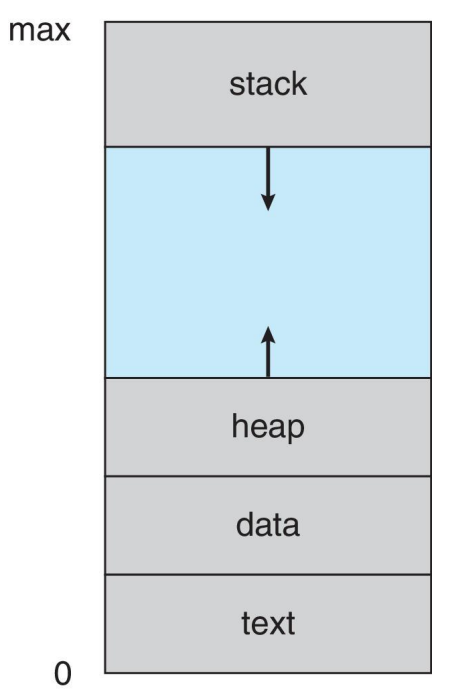
\includegraphics[width = .2\textwidth]{../res/imgs/processes/memory_layout.png}
    \caption{Spazio in memoria allocato per il processo dal sistema operativo.}
    \label{fig:memory_layout}
\end{figure}
Prima di tutto, il codice sorgente del programma viene caricato nella zona \textbf{text}. Dopo di che, nella parte dedicata ai dati (\textbf{data}) vengono salvate generalmente le variabili globali, che permangono per tutta la vita del processo. Sono infine presenti due parti: lo \textbf{stack} e l'\textbf{heap} che crescono in direzione opposta. Lo stack contiene dati temporanei come variabili locali mentre l'heap è utilizzato al fine di allocare la memoria dinamicamente durante la vita del programma\footnote{Come abbiamo visto con C++, heap e \textit{freestore} sono quasi dei sinonimi.}.

% 
\subsection{Process Control Block (PCB)}\label{PCB}
Ad ogni processo che è mandato in esecuzione è assegnata una particolare struttura dati dal sistema operativo, ovvero il \textit{Process Control Block} (figura \ref{fig:PCB}). Il PCB contiene diverse informazioni riguardanti il processo, in particolare:
\vspace{-5px}
\begin{enumerate}
\setlength{\itemsep}{-.15 em}
    \item Lo \textbf{stato} del processo;
    \item Informazioni sul \textbf{program counter}, in particolare è importante sapere se il processo è fermato temporaneamente e poi fatto ripartire più tardi;
    \item Valori dei registri, utili nel caso in cui un processo venga messo in pausa;
    \item Altre informazione riguardanti lo scheduling della CPU (vedi capitolo \ref{CPU scheduling}), come la priorità del processo;
    \item Informazioni per la gestione della memoria e dell'I/O.
\end{enumerate}
\begin{figure}[h]
    \centering
    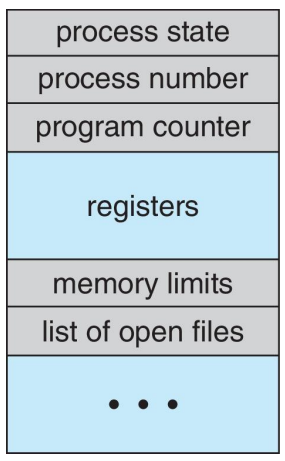
\includegraphics[width = .20\textwidth]{../res/imgs/processes/PCB.png}
    \caption{Rappresentazione del contenuto di un generico PCB.}
    \label{fig:PCB}
\end{figure}

\noindent In particolare, in \texttt{Linux}, nel PCB di un processo (che in Linux è chiamato \texttt{task}) sono presenti le seguenti informazioni: \texttt{pid} (numero assegnato al particolare processo), puntatori al processo genitore (che vedremo saranno utili nella fase di creazione di un processo), puntatori ai processi figli e altre informazioni come la lista dei file aperti. Quando un nuovo processo è creato in Linux, le sue informazioni sono detenute in una lista concatenata (\textit{doubly-linked list}) dove ogni nodo della lista è il PCB di un processo specifico (figura \ref{fig:process_table}). 
\begin{figure}[h]
    \centering
    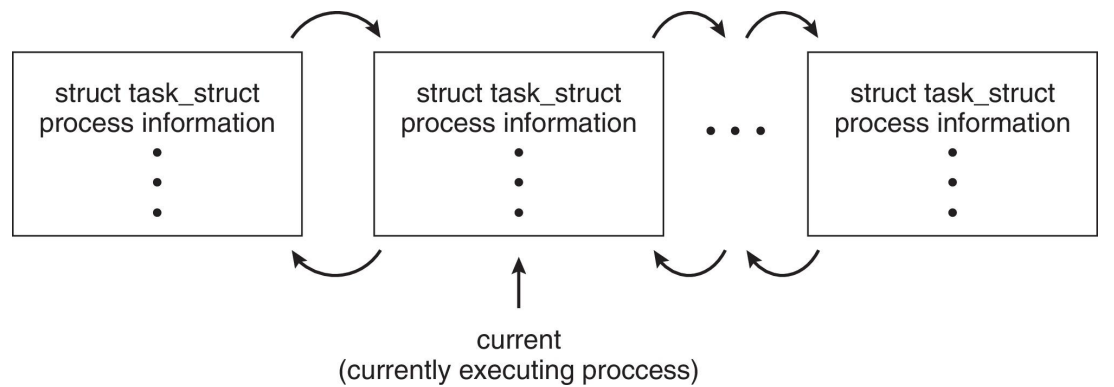
\includegraphics[width = .75\textwidth]{../res/imgs/processes/process_table.png}
    \caption{Lista concatenata che mantiene tutti i PCB dei processi (task) in Linux.}
    \label{fig:process_table}
\end{figure}
Al fine di andare a modificare delle informazioni del processo (come lo stato corrente) il sistema operativo scorre la lista e, dopo aver selezionato il PCB del processo desiderato, andrà a modificare il campo. 

% 
\section{Stati di un processo}
Durante l'intera vita del processo, questo passa in diversi stati (figura \ref{fig:process_life}). I principali sono:
\vspace{-5px}
\begin{enumerate}
\setlength{\itemsep}{-.15 em}
    \item \textbf{New}: il processo è appena stato creato;
    \item  \textbf{Ready}: il processo è pronto per essere eseguito, quindi non è ancora stato assegnato al processore e sta aspettando l'assegnazione;
    \item \textbf{Running}: dopo essere stato associato alla CPU il processo inizia ad essere eseguito. Come vedremo nel capitolo \ref{CPU scheduling} e successivi, il processo può essere interrotto e quindi ritorna allo stato ready;
    \item \textbf{Waiting}: se il processo deve aspettare qualche input da esterno si mette in attesa e una volta che riceve l'input ritorno nello stato ready;
    \item \textbf{Terminated}: una volta che il processo finisce la sua esecuzione, questo ovviamente termina e viene rimosso dalla CPU.
\end{enumerate}
\begin{figure}[h]
    \centering
    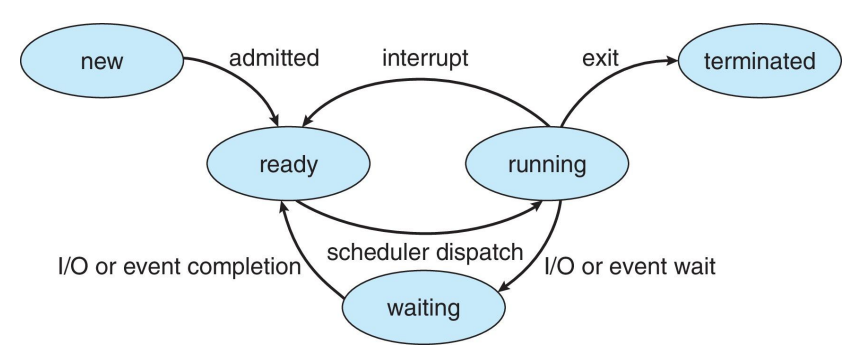
\includegraphics[width = .75\textwidth]{../res/imgs/processes/process_life.png}
    \caption{Gli stati della vita di un processo.}
    \label{fig:process_life}
\end{figure}

\noindent Lo stato \textit{ready} e lo stato \textit{wait} contengono delle code dove i processi attendono di essere eseguiti ovvero la \textbf{ready queue} e la \textbf{wait queue} che non sono altro che delle liste concatenate. Le liste contengono i PCB dei processi: il sistema operativo tiene traccia del primo e dell'ultimo processo nella lista al fine di riuscire a implementare le due code.  Possiamo inoltre suddividere i processi in due macro categorie:
\vspace{-5px}
\begin{itemize}
\setlength{\itemsep}{-.15 em}
    \item \textbf{CPU bound} che sono i processi che hanno un uso massiccio della CPU;
    \item \textbf{I/O bound}, ovvero processi che spendono la maggior parte del loro tempo in una situazione di wait per leggere o scrivere sulle periferiche.
\end{itemize}

% 
\subsection{Context switch}\label{context_switch}
Quando un processo A viene un rimosso dalla CPU, nel caso in cui sia stato interrotto per far spazio ad un altro processo B, è necessario salvare l'informazione del processo A in modo tale da poterlo sostituire con il processo B per poi, in un secondo momento, riuscire a ricaricare il processo A. Questa operazione è  detta \textbf{context switch} (figura \ref{fig:context_switch}) e viene effettuata in pochi microsecondi. Ciò nonostante se è effettuata in maniera molto frequente durante l'esecuzione di diversi processi può causare molto spreco di tempo: il context switch può quindi generare un \textbf{overhead} che va sicuramente preso in considerazione negli algoritmi di scheduling (capitolo \ref{CPU scheduling}).
\begin{figure}[h]
    \centering
    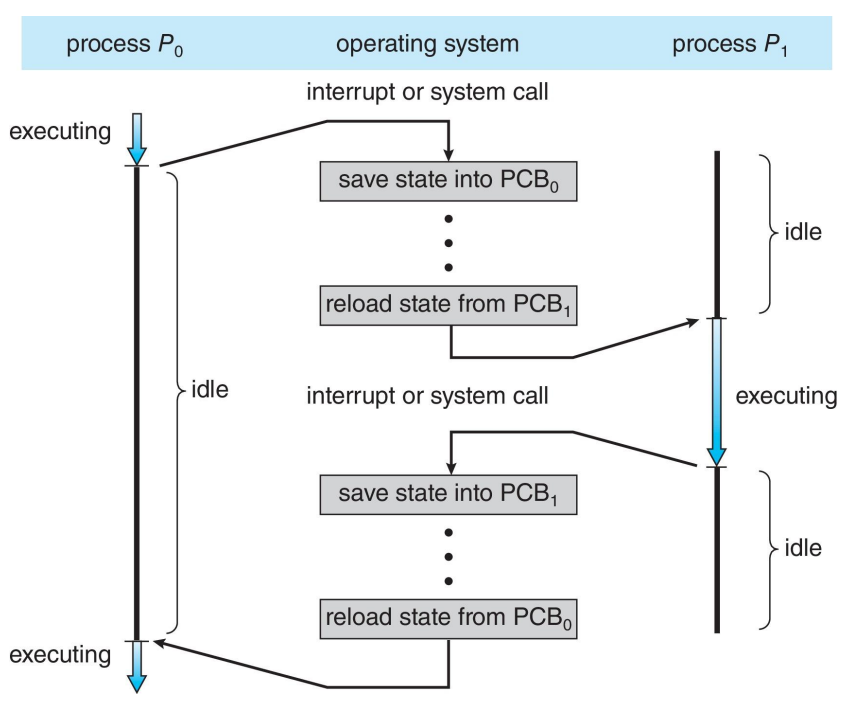
\includegraphics[width = .7\textwidth]{../res/imgs/processes/context_switch.png}
    \caption{Il context switch.}
    \label{fig:context_switch}
\end{figure}
È importante notare che il context switch tipicamente richiede anche un aggiuntivo utilizzo della memoria, che andremo a discutere nel capitolo \ref{main memory} quando discuteremo di \textit{paginazione} e \textit{swapping}.

% 
\subsection{Creazione di un processo}\label{creazione di un processo}
Al fine di creare un processo ce ne deve sempre essere uno iniziale (\textit{parent}) che genera il quello nuovo (\textit{child}). Ogni nuovo processo ha un identificativo, il \textbf{pid}, che distingue univocamente il processo creato. Al momento della creazione è possibile specificare alcune opzioni al fine di creare il processo child in un determinato modo. Prima tra tutte è l'opzione di \textbf{condivisione di risorse}, dove si può specificare se il figlio condivide le stesse risorse del genitore, un sottoinsieme oppure si può specificare che il figlio non condivida alcuna risorsa con il \textit{parent}. Inoltre si possono specificare le opzioni di \textbf{esecuzione}: si specifica se il figlio e il genitore possano essere eseguiti in maniera concorrente oppure se il \textit{parent} deve aspettare il termine dell'esecuzione del \textit{child}. Infine si può anche specificare lo \textbf{spazio degli indirizzi}, in particolare si sceglie se il figlio crea una copia identica della memoria utilizzata dal genitore oppure se carica un programma completamente nuovo.

Vediamo ora un esempio di creazione di un processo in \texttt{UNIX} (figura \ref{fig:fork}). Questo sistema operativo fornisce tre particolari \textit{system calls}:

\vspace{-5px}
\begin{itemize}
\setlength{\itemsep}{-.15 em}
    \item \texttt{fork()}: questa system call non fa altro che creare un processo. Il processo parent, dopo aver chiamato la funzione \texttt{fork()} viene duplicato. La funzione inoltre ritorna un valore intero, se questo valore è maggiore di zero vuol dire che ci troviamo all'interno del processo genitore; se invece il valore è zero vuol dire che il codice eseguito è all'interno del child. L'unico modo per distinguere se il processo è parent o child è attraverso il valore di ritorno di \texttt{fork}.
    \begin{figure}[h]
    \centering
    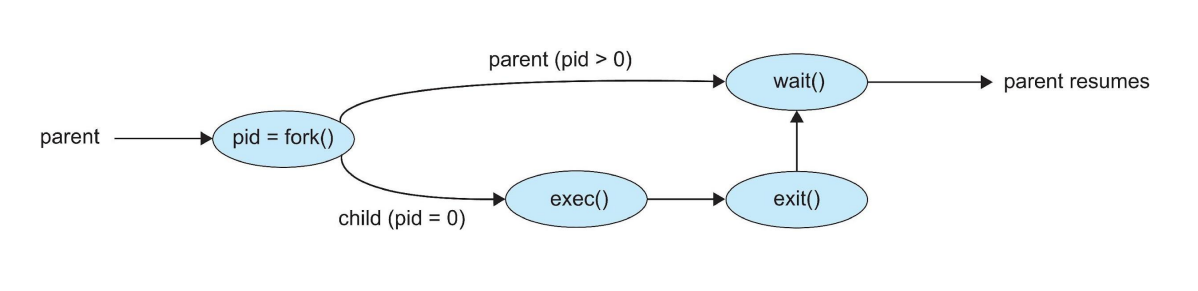
\includegraphics[width = .75\textwidth]{../res/imgs/processes/fork.png}
    \caption{Rappresentazione delle 3 \textit{system calls} fondamentali.}
    \label{fig:fork}
\end{figure}
    \item \texttt{exec()}: è una funzione utilizzata dal processo figlio nel caso in cui è necessario far partire un processo completamente diverso dal parent;
    \item \texttt{wait()}: è una systam call utilizzata dal genitore al fine di aspettare il termine dell'esecuzione del figlio.
\end{itemize}


%
\subsection{L'albero dei processi in Linux}
Come fa il sistema operativo a generare tutti i processi di cui ha bisogno? Ci deve sempre essere un processo iniziale, un programma all'inizio da cui tutti si genera. In particolare in Linux il primo processo da cui tutto è generato è chiamato \texttt{systemd} ed è il processo padre di tutti gli altri processi, quello il quale \texttt{pid} vale 1. Da \texttt{systemd}, \textit{forkando} processo dopo processo vengono generati tutti i processi necessari all'avvio del sistema, come il terminale, generando quindi un albero (figura \ref{fig:three_of_processes}).

\begin{figure}[h]
    \centering
    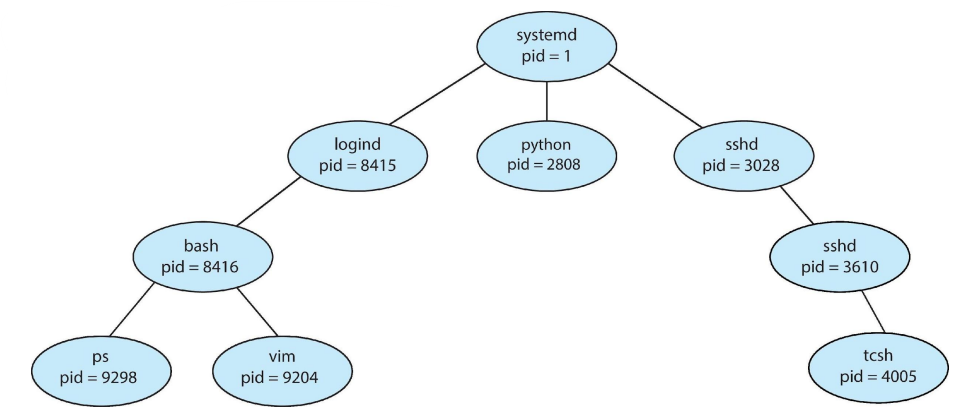
\includegraphics[width = .6\textwidth]{../res/imgs/processes/three_of_processes.png}
    \caption{L'albero dei processi generato da \texttt{systemd}.}
    \label{fig:three_of_processes}
\end{figure}

% 
\subsection{Terminazione di un processo}
Naturalmente, un processo può anche terminare. La terminazione del processo può essere spontanea (attraverso la \textit{system call} \texttt{exit}) e quindi il processo viene deallocato dal sistema operativo, oppure il processo può essere terminato dal genitore attraverso la system call \texttt{abort}. Questo di solito avviene quando il processo figlio supera il limite delle risorse allocate, quando la task che sta completando non è più richiesta oppure nel momento in cui il genitore termina e di conseguenza il sistema operativo termina anche i figli.

Come abbiamo visto in precedenza, esiste una funzione (\texttt{wait()}), che serve per evitare che il processo parent termini prima del processo child: la funzione infatti obbliga il parent ad aspettare che il child termini. Inoltre, se al termine di un processo child non c'è nessun processo parent che stava aspettando il termine del child, ci troviamo davanti ad un \textbf{processo zombie}. Infine, se il processo parent termina senza aspettare la terminazione del child, quest'ultimo è chiamato \textbf{orfano} e verrà terminato dal sistema operativo.

% 
\section{Comunicazione tra processi (IPC)}\label{IPC}
Passiamo ora a discutere i diversi modi per comunicare tra diversi processi. In alcuni casi avremo a che fare con processi indipendenti, altre volte invece necessiteremo di processi \textbf{cooperanti}. Per questi ultimi è necessario un modello di \textit{Inter-Process Communication}, chiamata anche \textbf{IPC}. In questo paragrafo ci occuperemo di due modelli: comunicazione tramite memoria condivisa e tramite il passaggio di messaggi.

% 
\subsection{Memoria condivisa}
Il primo modello di cui ci occuperemo è la tecnica di memoria condivisa. In questo modello, come possiamo notare anche dalla figura \ref{fig:shared_memory}, l'unica cosa di cui si fa carico il sistema operativo è l'assegnazione di una memoria che è condivisa tra i processi A e B.
\begin{figure}[h]
    \centering
    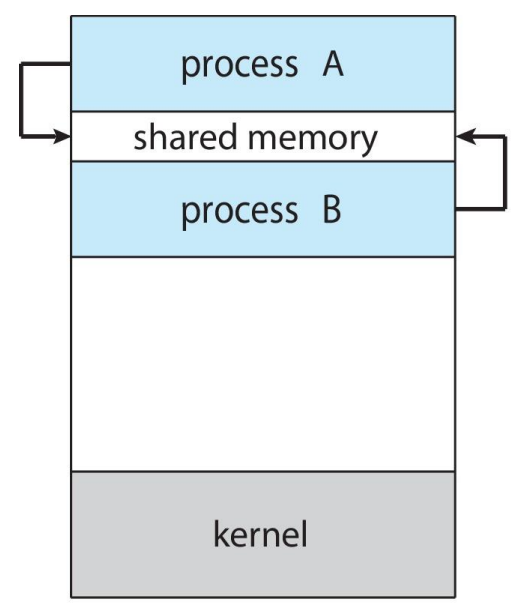
\includegraphics[width = .25\textwidth]{../res/imgs/processes/shared_memory.png}
    \caption{Il modello di memoria condivisa per IPC.}
    \label{fig:shared_memory}
\end{figure}
Ciò significa che la comunicazione è molto veloce tra i due processi in quanto non c'è nessun intermediario tra i due. Allo stesso tempo però è più facile che si generino errori come la sovrascrittura di valori e in genere problemi di sincronizzazione con i dati (come la \textit{race condition}, vedi capitolo \ref{sincronizzazione}) in quanto il sistema operativo non ha alcun tipo di controlla sulla memoria secondaria.

Partiamo ora da un esempio di questo modello al fine di ottenere informazioni più dettagliate: stiamo infatti parlando del problema \texttt{Producer - Consumer}. Ipotizziamo quindi che due processi abbiano dello spazio in memoria condiviso; la comunicazione attraverso questa memoria può avvenire in due modi:
\vspace{-5px}
\begin{itemize}
\setlength{\itemsep}{-.15 em}
    \item \textbf{unbounded}, ovvero che il produttore continua a generare dati da mettere nell'area condivisa, e che il consumatore continua ad utilizzare quei dati fino a che non finiscono (al più attende la creazione di altri dati).
    \item \textbf{bounded}, dove si ha un \textbf{buffer} che entrambi devono aspettare: il consumer attende che ci siano dati nel buffer e il producer aspetta nel momento in cui il buffer è pieno. 
\end{itemize}

% 
\subsection{Passaggio di messaggi}
In questo secondo caso invece il sistema operativo si prende carico di gestire la coda dei messaggi (\textbf{message queue}) che vengono scambiati tra i due processi (figura \ref{fig:message_passing}). In questo caso è il kernel che fa da intermediario tra i due e di conseguenza la velocità di comunicazione sarà ridotta dall'\textbf{overhead}.
\begin{figure}[h]
    \centering
    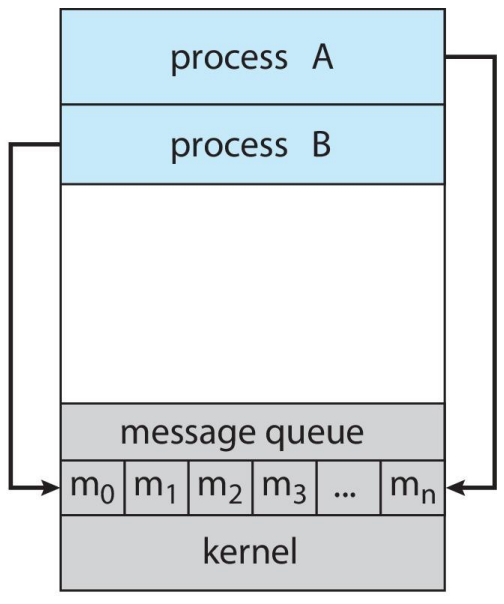
\includegraphics[width = .25\textwidth]{../res/imgs/processes/message_passing.png}
    \caption{Il modello di memoria condivisa per IPC.}
    \label{fig:message_passing}
\end{figure}
Allo stesso tempo però il kernel garantisce la sincronizzazione e la correttezza tra i messaggi scambiati e di conseguenza è un modello più sicuro. 

Discutiamo ora più dettagliatamente questo modello. In particolare, sono fornite due operazioni fondamentali: \texttt{send(message)} e \texttt{recive(message)}. Ciò nonostante la comunicazione di tali messaggi fa sorgere diversi dubbi e domande legate alla progettazione: come sono stabilite le connessioni? qual è la sua capacità? è unidirezionale o bidirezionale? la dimensione del messaggio è fissa o variabile? un collegamento è associato solo a 2 processi o a più? Per rispondere a queste domande andiamo a vedere l'implementazione di questo modello che può essere di due tipi.

Quando si parla di comunicazione \textbf{diretta}, si intende che i processi specifichino esplicitamente il destinatario del messagio: \texttt{send(Q, message)} e \texttt{recive(P, message)}. Nella comunicazione \textbf{indiretta} invece si ha a che fare con un \textbf{buffer}, chiamato anche porta, il quale ha un ID unico tra gli altri. In questa implementazione due processi si possono parlare solo se condividono questo buffer (\textbf{mailbox}). Se più processi condividono la stessa mailbox si ha quindi un link che collega diversi processi, inoltre attraverso questa porta il collegamento è bidirezionale in quanto un processo può sia spedire un messaggio che riceverlo. Con la comunicazione indiretta le primitive però sono diverse: una volta creata la porta (chiamiamola \texttt{A}, per comodità), al fine di scambiare i messaggi è necessario utilizzare le operazioni \texttt{send(A, message)} e \texttt{recive(A, message)}.
